\chapter{Experiments}\label{ch:experiments}

We use the same cINN normalizing flow architecture, spectral-normalized GAN (SN-GAN)~\cite{sngan} discriminator architecture, and
Adam optimizer parameters between all experiments.
The details of the common model and optimizer hyperparameters are listed in Appendix~\ref{ch:model-and-optimizer-hyperparameters}.

We split the dataset into 2019 and 2020 solely for training and hold out 2021 for evaluation.
We follow a strict backtesting procedure where a model producing forecasts for an upcoming market-day has only been
trained on data that would be available to a real participant prior to the market-day.

All models in this work were trained on an NVIDIA GTX 1060--6GB GPU using Python v3.10.8 and PyTorch v1.13.0.
While GPU training allowed larger batch sizes and accelerated training times, often under 10 minutes, these
models can be trained on CPU with smaller batch sizes, often taking between 10-30 minutes (tested on an AMD
Ryzen 3700x @ 3.6GHz with 16GB RAM and a 2020 Intel i7 @ 2.3GHz 13-inch Apple Macbook-Pro with 16GB RAM).

\section{Capturing Non-Stationary Prices}\label{sec:capturing-non-stationary-prices}

We first investigate the ability of our model to capture how energy price distributions change over time.
All experiments in this section use a vanilla normalizing flows model, ignoring the adversarial loss term by setting
$\lambda_{\text{ADV}} = 0$ in~\eqref{eq:flowgan_loss}.
As energy prices are fundamentally driven, we can ascribe changes in the price distributions to changes in factors such
as \textit{grid topology}, \textit{fuel prices}, \textit{population and load patterns}, \textit{generator outages},
\textit{renewable penetration}, \textit{generation mix}, \textit{weather patterns}, etc.
We note that a much of the variation in energy prices can be explained by changes in the fundamentals of our dataset,
for example the relationship between energy prices and gas prices as shown in Figure.~\ref{fig:price_gas_hist},
seasonal load patterns as shown in Figure~\ref{fig:weekly_load}, or seasonal generation mixes shown in
Figure~\ref{fig:weekly_windgen}.
However, while a well calibrated model can capture the complex, nonlinear relationships of these quantities with the powerful
capacities provided by deep learning methods, these interactions change over time and with respect to inaccessible,
such as grid topology.

\begin{figure}[htbp]
    \caption[Relationship between quarterly aggregated day-ahead prices and natural gas prices]{
        Relationship between day-ahead LMPs and natural gas prices.
        The left-y-axis and histograms show the distribution of Chicago Hub DA-LMPs aggregated
        on a quarterly basis.
        The right-y-axis and black dots-and-flyers show quaterly aggregate natural gas prices at TETCO-M3
        where the dots represent the mean price and the upper, lower flyers represent the $75^{\text{th}}$ and
        $25^{\text{th}}$ percentiles respectively.
        Observe the relationship between the mean and tails of the gas price distributions and the shape
        of the DA price distributions over time.
    }
    \begin{center}
        \setlength{\fboxsep}{0pt}%
        \setlength{\fboxrule}{1pt}%
%        \fbox{
        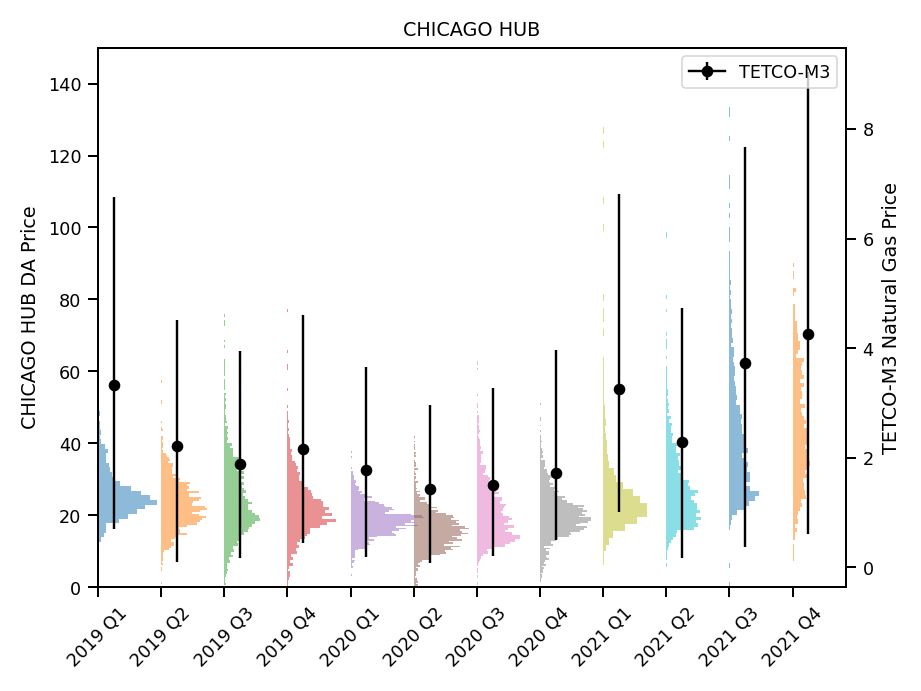
\includegraphics[width=120mm]{figs/chicago_hub_tetco_dists}
%        }
    \end{center}
    \label{fig:price_gas_hist}
\end{figure}

\begin{figure}[htbp]
    \caption[Total aggregate load v.s. day-ahead prices]{
        The relationship between day-ahead LMPs and seasonal load patters.
        The left-y-axis and blue curve shows mean total load forecast in PJM aggregated on a weekly basis.
        The right-y-axis and orange curve show the weekly aggregate mean Chicago Hub DA-LMP.
    }
    \begin{center}
        \setlength{\fboxsep}{0pt}%
        \setlength{\fboxrule}{1pt}%
%        \fbox{
        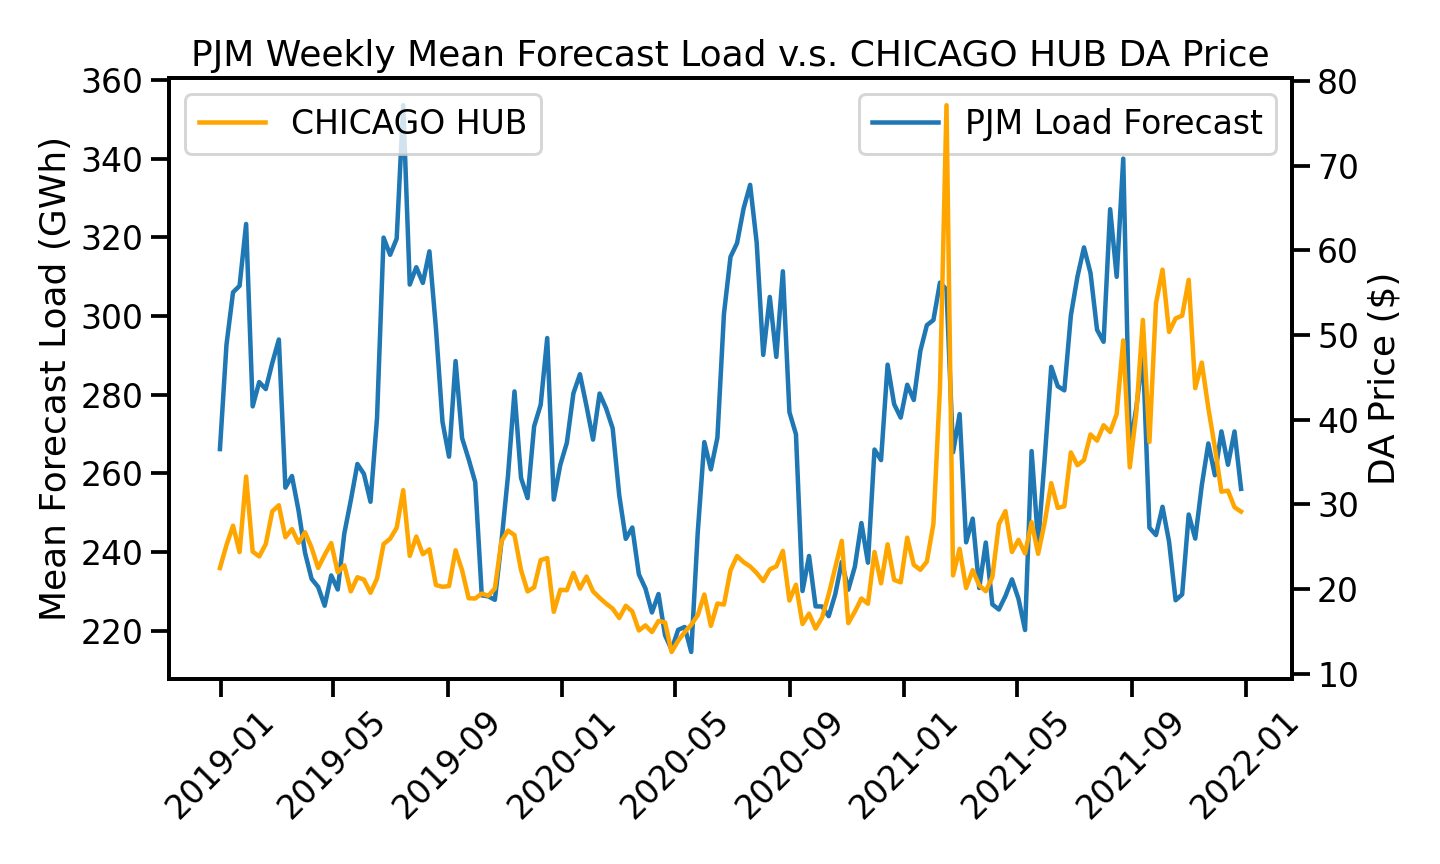
\includegraphics[width=120mm]{figs/load_vs_price}
%        }
    \end{center}
    \label{fig:weekly_load}
\end{figure}

\begin{figure}[htbp]
    \caption[Total aggregate wind generation v.s. day-ahead prices]{
        The relationship between day-ahead LMPs and seasonal wind generation patters.
        The left-y-axis and blue curve shows mean total wind generation forecast in PJM aggregated on a weekly basis.
        The right-y-axis and orange curve show the weekly aggregate mean Chicago Hub DA-LMP.
    }
    \begin{center}
        \setlength{\fboxsep}{0pt}%
        \setlength{\fboxrule}{1pt}%
%        \fbox{
        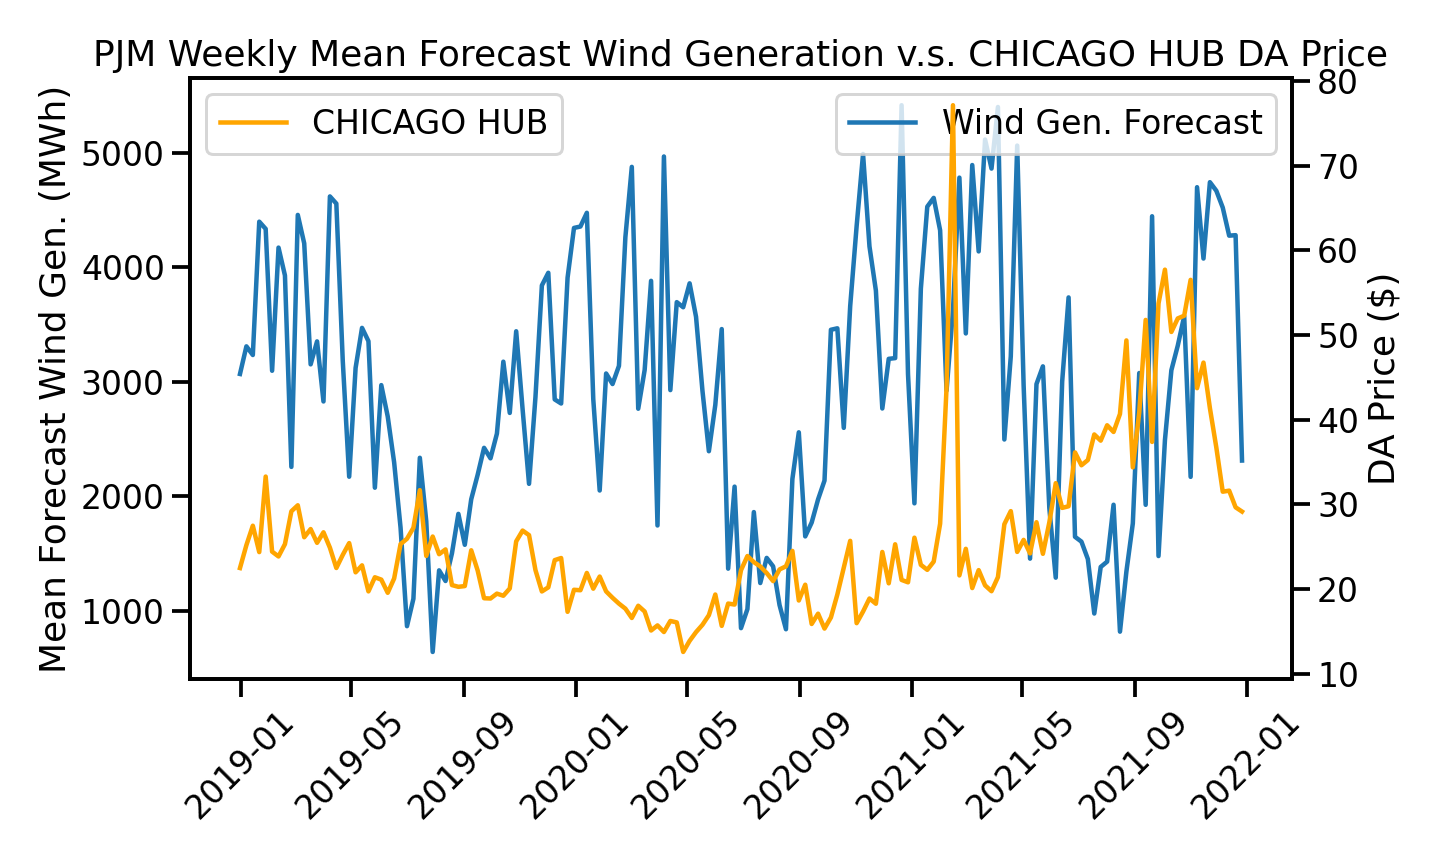
\includegraphics[width=120mm]{figs/windgen_vs_price}
%        }
    \end{center}
    \label{fig:weekly_windgen}
\end{figure}

As is common in energy price forecasting literature, and timeseries forecasting literature in general, we first
investigate the benefits of \textit{recalibration}, which is simply adjusting the parameters of the model as more
recent information becomes available.
The recalibration process is defined as retraining the model from scratch every $T$ market-days, where
$T \in \mathbb{N}^+$ is a hyperparameter.
Setting $T=1$ is equivalent to re-training the model from scratch each day before trade generation and submission and
setting $T \geq 365$ is equivalent to never recalibrating the model.
For market-days between recalibration dates the model parameters stay the same and are not updated when new information
comes in.

We sweep over multiple values of $T < 365$ and compare against a baseline ``fixed'' model that is never recalibrated
over the 2021 validation set.
Unsurprisingly, the results, shown in Table~\ref{tab:recalibration}, make it clear that recalibrating model parameters
more often produces better results.
From these results, it is recommended to recalibrate the model as often as possible, i.e. daily.
For the remainder of the experiments in this work the recalibration period is fixed to 14 days as this was observed
value to be good tradeoff between performance and computation time when running experiment back-tests.

\begin{table}[htb]
    \caption[Results of parameter recalibration]{
        Comparison of various model recalibration intervals.
    }
    \begin{center}
        \begin{tabular}{||c|c|c|c||} \hline
        Recalibration Interval ($T$) & Median NLL (-)  & $99\%$ NLL (-) & mCRPS (-)  \\	% footnote symbols!
        \hline \hline
        \geq 365  &         -26.337  &         86.574  &        10.392  \\ \hline
        90        &         -41.724  &         65.773  &         9.413  \\ \hline
        30        & \textbf{-48.487} &         73.809  &         8.463  \\ \hline
        14        &         -44.127  & \textbf{63.294} & \textbf{7.508} \\ \hline
        \end{tabular}
        \\ \rule{0mm}{5mm}
    \end{center}
    \label{tab:recalibration}
\end{table}

Beyond parameter recalibration, when dealing with non-stationary prices in energy price forecasting literature, and
again timeseries forecasting literature in general, recent data is more informative to upcoming forecasts than data
further back in history.
For example, if forecasting energy prices for the upcoming week there is intuitive reasoning that data from the most
recent two weeks in history is a more informative dataset compared to an arbitrary two weeks from two years ago.
To capture this, practitioners often use a \textit{rolling-window} of data, whereby only data from the most
recent $R \in \mathbb{N}^+$ examples in history are used to estimate model parameters.
While this technique may work well for models with few parameters, we found these methods to be generally
unsuitable for our work, as shown in Table~\ref{tab:rolling_window} where $R$ represents the number of market-days in our
training window.
We believe this is caused by the deep learning model not having enough data to train and generalize well.
Reducing the dataset significantly results in the model becoming significantly over-parameterized and more likely to
over fit to the limited data in training windows.

\begin{table}[htb]
    \caption[Results of reducing the training window]{
        Comparison multiple sizes of rolling training windows.
    }
    \begin{center}
        \begin{tabular}{||c|c|c|c||} \hline
        Window Size ($R$) & Median NLL (-)  & $99\%$ NLL (-) & mCRPS (-)  \\	% footnote symbols!
        \hline \hline
        \infty &         -44.127  & \textbf{63.294} & \textbf{7.508} \\ \hline
        90     & \textbf{-47.907} &        283.582  &         8.327  \\ \hline
        30     &         -20.01   &       1004.566  &        13.73   \\ \hline
        14     &          25.551  &     418573.25   &        15.43   \\ \hline
        \end{tabular}
        \\ \rule{0mm}{5mm}
    \end{center}
    \label{tab:rolling_window}
\end{table}

Instead, we \textit{emphasize} the most recent or most important training observations for the upcoming forecast window.
We note two possible ways one could go about this,

\begin{enumerate}
    \item Construct a set of weights $\left\{ w_i \right\}_{i=1}^K$ such that $w_i \in [0, 1]$ and
    $\sum_{i=1}^K w_i = 1$ where $K$ is the number of observations in the training set.
    Let weight $w_i$ be the probability of drawing training observation $i$, then we can perform random sampling with
    replacement on our training set to train our model with emphasis on observations with greater weight.
    \item Train on all $K$ observations in history.
    Then, construct a subset of $K' < K$ training observations and \textit{fine-tune} the trained model parameters on
    the subset of data.
\end{enumerate}

We pursue only the fine-tuning approach here.
Fine-tuning is implemented by taking the subset of training observations to be the $R$ most recent
days in history at the time of model recalibration.
After recalibrating the model parameters on all training examples, the optimized learning rate is reduced and training
is continued on the subset of $R$ most recent days in history.
Following from previous results, recalibration and fine-tuning of parameters is performed every 14 market-days with no
parameter updates between recalibrations.
We sweep over multiple values of $R$ and compare a baseline model which is only recalibrated but not fine-tuned.
The results for the proposed fine-tuning strategy are presented in Table~\ref{tab:finetune}.

\begin{table}[htb]
    \caption[Results of rolling window fine-tuning]{
        Comparison of fine-tuning rolling window sizes
    }
    \begin{center}
        \begin{tabular}{||c|c|c|c||} \hline
        Window Size ($R$) & Median NLL (-)  & $99\%$ NLL (-) & mCRPS (-)  \\	% footnote symbols!
        \hline \hline
        None &          -44.127  & \textbf{63.294} &         7.508  \\ \hline
        14   &          -49.839  &         65.27   & \textbf{5.723} \\ \hline
        45   &  \textbf{-52.346} &         66.59   &         6.686  \\ \hline
%        90   & xxx & xxxx & xxx \\ \hline
        \end{tabular}
        \\ \rule{0mm}{5mm}
    \end{center}
    \label{tab:finetune}
\end{table}

Observe that fine-tuning on the most recent examples in history improves both model fit measured via
median NLL and forecast accuracy measured via mCRPS\@.
Moreover, reducing the size of the fine-tuning dataset to only the most relevant training examples (in this case more
recent $\implies$ more relevant) has the largest impact on results.
Future work may investigate a better selection method for the fine-tuning dataset to obtain important training
observations beyond the most recent days in history (for example, weeks with similar weather and load patterns).

\section{Improving Sampling Tasks with Adversarial Loss}\label{sec:improving-sampling-tasks}

Next, the impact of including the adversarial loss term, $\mathcal{L}_{\text{ADV}}$, in the hybrid loss function and
how it specifically affects sampling performance of the model are investigated.
The 14-day recalibration and 14-day fine-tuning window methods are utilized in the following experiments.
A range of values for $\lambda_{\text{ADV}} > 0$ are swept over and compared against a baseline model without adversarial
loss, the results are shown in Table~\ref{tab:ganloss}.

\begin{table}[htb]
    \caption[Results of including adversarial loss]{
        Comparison of fine-tuning rolling window sizes
    }
    \begin{center}
        \begin{tabular}{||c|c|c|c||} \hline
        $\lambda_{\text{ADV}}$ & Median NLL (-)  & $99\%$ NLL (-) & mCRPS (-)  \\	% footnote symbols!
        \hline \hline
        0   &         -49.839  &         65.27   &         5.723 \\ \hline
        0.1 &         -50.02   &         65.103  &         5.637 \\ \hline
        1   & \textbf{-50.442} &         65.176  &         5.569 \\ \hline
        10  &         -50.394  & \textbf{62.854} & \textbf{5.309} \\ \hline
        \end{tabular}
        \\ \rule{0mm}{5mm}
    \end{center}
    \label{tab:ganloss}
\end{table}
The inclusion of adversarial loss improves the mCRPS metric.
To investigate why, first note the sensitivity of our CRPS estimator to outliers in our samples.
Consider the empirical c.d.f for a arbitrary distribution represented by a set of finite samples, if some of samples
are extreme outliers then they will carry a non-trivial mass under the tail of the distribution.
Depending on the number and magnitude of the outliers this tail may over-estimate the tail of the true distribution
resulting in a degraded CRPS estimation.

To illustrate this issue with an example, let $\mathcal{U} \sim \text{Gumbel}(\mu=0, \beta=1)$ with realizations $u$.
The empirical c.d.f. $\hat{F}_\mathcal{U}$ is constructed by drawing 500 samples.
A second c.d.f. $\hat{F}'_\mathcal{U}$ is constructed using the same examples, however, with a single outlier observation
$u=10,000$ added to the set of samples.
For an observation at $y=0$, the CRPS estimators are computed to be $\widehat{CRPS}_{\hat{F}_\mathcal{U}}(0) = 0.3331$
and $\widehat{CRPS}_{\hat{F}'_\mathcal{U}}(0) = 0.3748$ respectively.
Clearly, extreme outliers have a detrimental effect on estimated CRPS metrics.

%\begin{figure}[htbp]
%    \caption[Example CRPS calculation of a standard Gumbel distribution]{
%        The CRPS of a standard Gumbel distribution, $\text{Gumbel}(\mu=0, \beta=1)$, estimated by 500 samples is
%        calculated against an observation at $0$.
%        The top figure shows the emperical cdf of the samples while the curve in the bottom plot shows the squared error
%        between the emperical cdf of our samples and the cdf formed by the true observation.
%        The CRPS itself is the area under the bottom curve shown in grey.
%    }
%    \begin{center}
%        \setlength{\fboxsep}{0pt}%
%        \setlength{\fboxrule}{1pt}%
%%        \fbox{
%        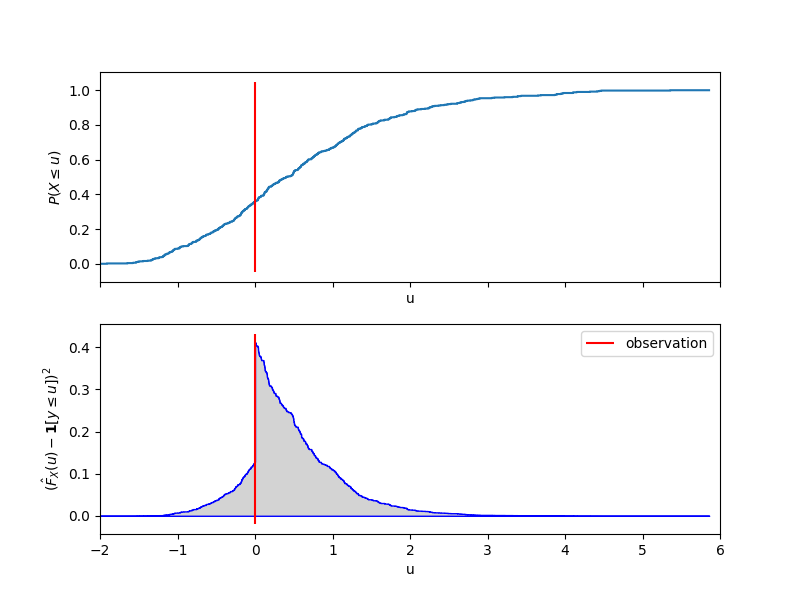
\includegraphics[width=120mm]{figs/gumbel_crps}
%%        }
%    \end{center}
%    \label{fig:gumbel_crps}
%\end{figure}

When observing the sample distribution drawn from a trained price density model, extreme outliers can be readily noticed.
Figure~\ref{fig:badsamples} shows 500 samples which estimate the joint density forecast between two price nodes
marginalized out from a larger joint forecast.
Most samples are indistinguishable from one-another and located near the origin as expected, however,
observe the small number of samples whose magnitudes are on the order of \$$10^7$.
It is clear how these samples would severely degrade the CRPS metrics of this forecast.

\begin{figure}[htbp]
    \caption[Forecast joint distribution with extreme outliers]{
        A marginalized joint distribution forecast between WESTERN HUB and AEP GEN HUB price nodes.
        Note the outliers with values on the order of magnitude of \$$10^7$ which exceed both
        reasonable price expectations and hard price limits enforced by PJM.
    }
    \begin{center}
        \setlength{\fboxsep}{0pt}%
        \setlength{\fboxrule}{1pt}%
%        \fbox{
        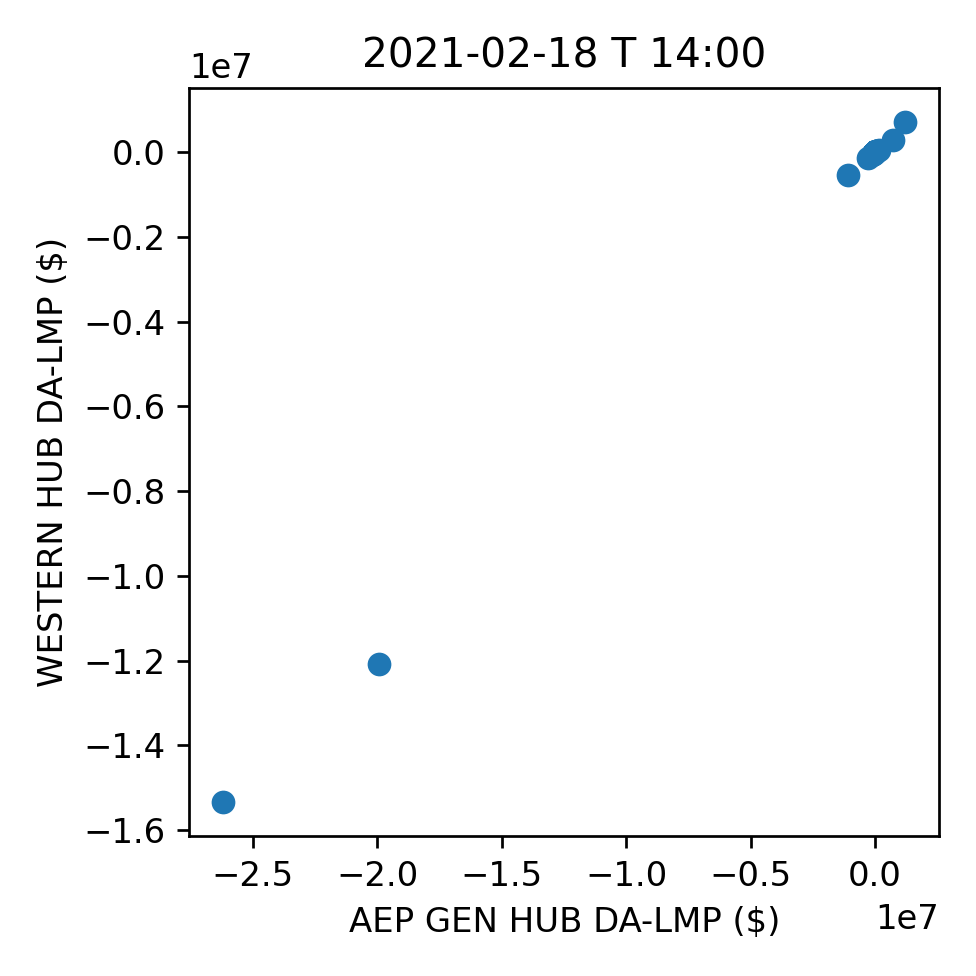
\includegraphics[width=100mm]{figs/bad_samples}
%        }
    \end{center}
    \label{fig:badsamples}
\end{figure}

To determine if adversarial loss address this problem in particular, it is necessary to quantify the frequency of extreme
outliers.
Starting with the matrix $\mathbf{X}_t \in \mathbb{R}^{r \times n}$ representing $r$ samples for a forecast at time
$t$ over $n$ price nodes.
The sample covariance matrix for $\mathbf{X_t}$ associated eigenvalues ${\sigma_1 \dots \sigma_n}$ are computed.
Let the \textit{total uncertainty} (TU) of our forcast be defined as

\begin{equation*}
    \text{TU}_\mathbf{X_t} = \sum_{i=1}^{n} \sqrt{\sigma_i},
    \label{eq:total_uncertainty}
\end{equation*}

which can be interpreted as the cumulative standard deviations in price along each orthogonal dimension in some rotated
price space.
Next, the \textit{excess uncertainty} (EU) is defined as a binary indicator on the total uncertainty exceeding a set
threshold,

\begin{equation*}
    \text{EU}_{\mathbf{X}_t} = \mathbbm{1}_{\left[ TU_{\mathbf{X}_t} \geq 1000 \right]},
    \label{eq:excess_unc}
\end{equation*}
where 1000 is chosen as the threshold because day-ahead prices rarely exceed the low hundreds of dollars on more than a
handful of nodes at any time, thus this threshold expected to be rarely exceeded under normal market conditions.

Counting the total excess uncertainty over all forecasts on the validation set then provides a metric for the
frequency of outliers,

\begin{equation*}
    \text{Total Excess Uncertainty} = \sum_{t=1}^{T} EU_{\textbf{X}_t}.
    \label{eq:total_unc}
\end{equation*}
Comparison of the total excess uncertainty for various forecasting strategies are shown in Table~\ref{tab:total_unc}.
The inclusion of adversarial loss ($\lambda_{\text{ADV}} = 10$) reduces the occurrences of forecasts with excessive
uncertainty likely improving the CRPS metrics forecasts.

\begin{table}[htb]
    \caption[Count of forecasts with excessive uncertainty over various models]{
        The total excessive uncertainty is captured for four models over the training set.
        Recalibration and fine-tuning sizes are both set to $14$, $\lambda_{\text{ADV}} = 10$.
        The model denoted as \textit{none} has no recalibration, fine-tuning, or adversarial loss.
        Strategies are assumed to be ommitted unless specified in the model name.
    }
    \begin{center}
        \begin{tabular}{||c|c||} \hline
        Model Strategy & Total Excess Uncertainty  \\	% footnote symbols!
        \hline \hline
        None                            & 34 \\ \hline
        Recal.                          & 180 \\ \hline
        Recal. + Fine-tune              & 379 \\ \hline
        Reval. + Fine-tune + Adv. Loss  & 72 \\ \hline
        \end{tabular}
        \\ \rule{0mm}{5mm}
    \end{center}
    \label{tab:total_unc}
\end{table}

We hypothesize this effect is due to the ``contraction'' of the reference density when transforming to the target
density under adversarial loss due to naturally arising mode-collapse phenomena.
When using a normalizing flow model as the generator of a GAN, mode-collapse can be understood as the
contraction of the target density to a small neighborhood in the target-space\footnote{
    Indeed, results from the original FlowGAN work~\cite{flow_gan} show an exploding $\mathcal{L}_{\text{MLE}}$ when
    trained only on $\mathcal{L}_{\text{ADV}}$ despite high-quality samples still being drawn which furthers this
    density contraction hypothesis.
} as demonstrated in Figure~\ref{fig:mode_collapse}.

\begin{figure}[htbp]
    \caption[Mode-covering and mode-collapsed density estimators on synthetic data]{
        A comparison of a mode-covering and mode-collapsed density estimators.
        \textbf{Left:} the true multi-modal distribution.
        \textbf{Center:} a mode-covering Flow-GAN density estimator trained using only $\mathcal{L}_{\text{MLE}}$ loss.
        \textbf{Right:} a mode-collapsed Flow-GAN density estimator trained using only $\mathcal{L}_{\text{ADV}}$ loss.
    }
    \begin{center}
        \setlength{\fboxsep}{0pt}%
        \setlength{\fboxrule}{1pt}%
%        \fbox{
        
\includegraphics[width=120mm]{figs/mode-collapse}
%        }
    \end{center}
    \label{fig:mode_collapse}
\end{figure}

This contracting behavior is believed to regularize the mapping of the normalizing flow model in the low-density tails
of the estimated target density by pulling density from the tails of the distribution in towards the modes.
Figure~\ref{fig:flow_circs} shows a synthetic distribution whose density transport map is learned by a normalizing flow model.
Observe the warping of the reference domain by a set of concentric circles drawn in the reference space and their
subsequent mappings in the target space.
Near the tails of the target density there is excessive warping of the reference domain as it becomes more
difficult for the normalizing flow model to accurately capture low-probability tail behavior due to a lack of training
observations and penalty for excessive warping of the domain.
Extrapolating to higher dimensions, this warping would likely cause the occasional sample in reference space to be
mapped to an outlier in the target space due to a manifestation of the curse of dimensionality.
Thus, the hypothesized regularizing properties of adversarial loss would rein in excessive warping under an
estimated mapping.
In the context of our work it is enticing to refer to the inclusion of adversarial loss as \textit{adversarial
regularization} due to the properties observed.

\begin{figure}[htbp]
    \caption[Illustration of domain warping for synthetic 2-d distribution]{
        The warping of the reference domain under the push-forward opertion of a trained normalizing flow model with
        with three affine-coupling layers.
        \textbf{Left:} Reference samples shown in blue and concentric circles in the reference domain
        drawn in black.
        \textbf{Right:} Samples pushed-forward into the target space and the same concentric circles
        warped in the target domain.
    }
    \begin{center}
        \setlength{\fboxsep}{0pt}%
        \setlength{\fboxrule}{1pt}%
%        \fbox{
        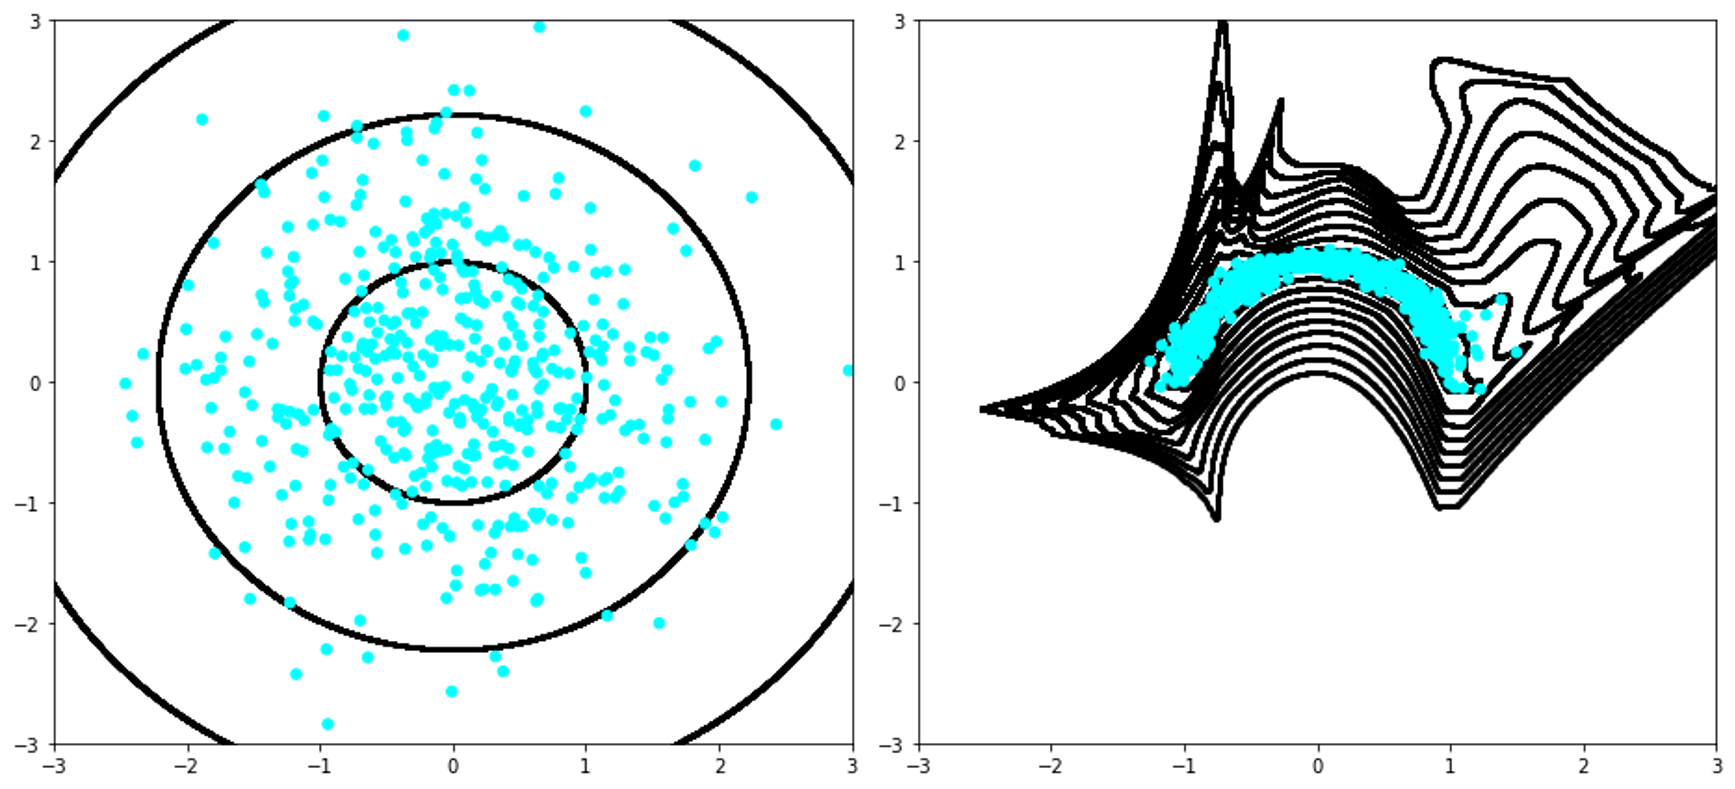
\includegraphics[width=120mm]{figs/nf_circs_cropped}
%        }
    \end{center}
    \label{fig:flow_circs}
\end{figure}

\section{Comparison Against Baselines}\label{sec:comparison-against-baselines}

Finally, we compare our proposed probabilistic forecasting methodology (including recalibration, fine-tuning, and
adversarial regularization) against several baseline traditional point forecasting methods.
Comparisons are first provided against two open source state-of-the-art energy price forecasting models in literature
found in the \texttt{epf-toolbox}~\cite{epftoolbox} python library.
We compare against both the modified \textit{lasso estimated auto-regressive} (EPF-LEAR) model and modified
\textit{deep neural network} (EPF-DNN) model as described in Section~\ref{sec:baselines}.
Note, a significant downside to these models is they are only defined for single price nodes, making multi-node
forecasts significantly more expensive to obtain and the resulting forecasts would likely fail sufficiently to capture
the joint structure between node prices.
As such, only comparisons at a select few price nodes are performed.
For each price node, a single DNN model and 24 hourly LEAR models a constructed.
Univariate density forecasts for each price are obtained by marginalizing out samples from the entire joint density
forecast.
To match the parameter recalibration of our proposed models, the same training and recalibration procedures are followed
with both the EPF-LEAR and EPF-DNN models.
Comparisons between the CRPS of our probabilistic forecasts (cINN) against the MAE of the EPF-DNN and EPF-LEAR forecasts
are shown in Table~\ref{tab:epf_comp}.
The proposed density forecasting method produces more accurate forecasts than state-of-the-art point forecasting methods.
Note, beyond greater forecast accuracy our proposed methodology also captures joint structures between
price nodes and uncertainty in forecasts which non-probabilistic forecasts fail to provide.

\begin{table}[htb]
    \caption[Comparison of proposed forecasts v.s. open-source state-of-the-art methods]{
        Comparison of forecast accuracy between our probabilistic forecasting strategy and state-of-the-art
        models from the $\texttt{epf-toolbox}$~\cite{epftoolbox} python library over single price nodes.
    }
    \begin{center}
        \begin{tabular}{||c|c|c|c||} \hline
        \diagbox{Price Node}{Model} & EPF-LEAR (MAE) & EPF-DNN (MAE) & cINN (mCRPS)  \\	% footnote symbols!
        \hline \hline
        CHICAGO HUB    & 6.622 & 6.231 & \textbf{5.341} \\ \hline
        DOMINION HUB   & 7.077 & 6.565 & \textbf{6.174} \\ \hline
        EASTERN HUB    & 7.095 & 7.526 & \textbf{6.087} \\ \hline
        NEW JERSEY HUB & 4.923 & 5.025 & \textbf{3.983} \\ \hline
        OHIO HUB       & 6.444 & 6.119 & \textbf{5.558} \\ \hline
        \end{tabular}
        \\ \rule{0mm}{5mm}
    \end{center}
    \label{tab:epf_comp}
\end{table}

Next, the proposed density forecasting methodology is compared against the commercial OPF solver.
The solver only produces point forecasts on a subset of 14 of our price nodes, thus the joint
density forecast on those specific nodes is marginalized out from the larger joint density.
Again, the MAE of the OPF forecasts is compared against the mCRPS of the probabilistic forecast with results shown
in Table~\ref{tab:opf_comp}.
The probabilistic forecasting strategy is more accurate than the commercial, physics-based price
forecasting tool, again with the added benefit of information-rich joint probabilistic forecasts as opposed to
low-information point forecasts.

\begin{table}[htb]
    \caption[Comparison of proposed forecasts v.s. commercial optimal powerflow solver]{
        Comparison of forecast accuracy between our proposed probabilistic forecasting strategy and a commercial
        OPF solver over a subset of 14 prices nodes.
    }
    \begin{center}
        \begin{tabular}{||c|c|c||} \hline
        Model & MAE (-) & mCRPS (-)  \\	% footnote symbols!
        \hline \hline
        OPF  & 6.666 &           -    \\ \hline
        cINN &   -   & \textbf{5.435} \\ \hline
        \end{tabular}
        \\ \rule{0mm}{5mm}
    \end{center}
    \label{tab:opf_comp}
\end{table}

Figure~\ref{fig:forecast_timeseries} illustrates forecasts from our joint density method and the three baseline methods
against observed DA prices on a single node over two time intervals in 2021.
Observe how the uncertainty in our proposed density forecasting method changes with respect to market conditions.
Also note that beyond the mean forecast and 95\% confidence intervals, each forecast is a complex probability density
function as shown in Figure~\ref{fig:univar_dens}.

\begin{figure}[htbp]
    \caption[Timeseries of observed v.s. forecast prices]{
        Forecasts from the proposed probabilistic forecasting methodology, EPF-LEAR, EPF-DNN, and OPF baselines
        against the true NEW JERSEY HUB DA LMPs over two five-day intervals in 2021.
        (a) forecasted and observed LMPs over five-days during an extreme winter weather event in Texas
        that caused unprecendented price action in PJM.
        (b) forecasted and observed LMPs over a typical five-day interval in the summer.
        Note the differences in uncertainty and intra-day price action captured by the probabilistic forecasts
        during the different market conditions.
    }
    \begin{center}
        \setlength{\fboxsep}{0pt}%
        \setlength{\fboxrule}{1pt}%
%        \fbox{
        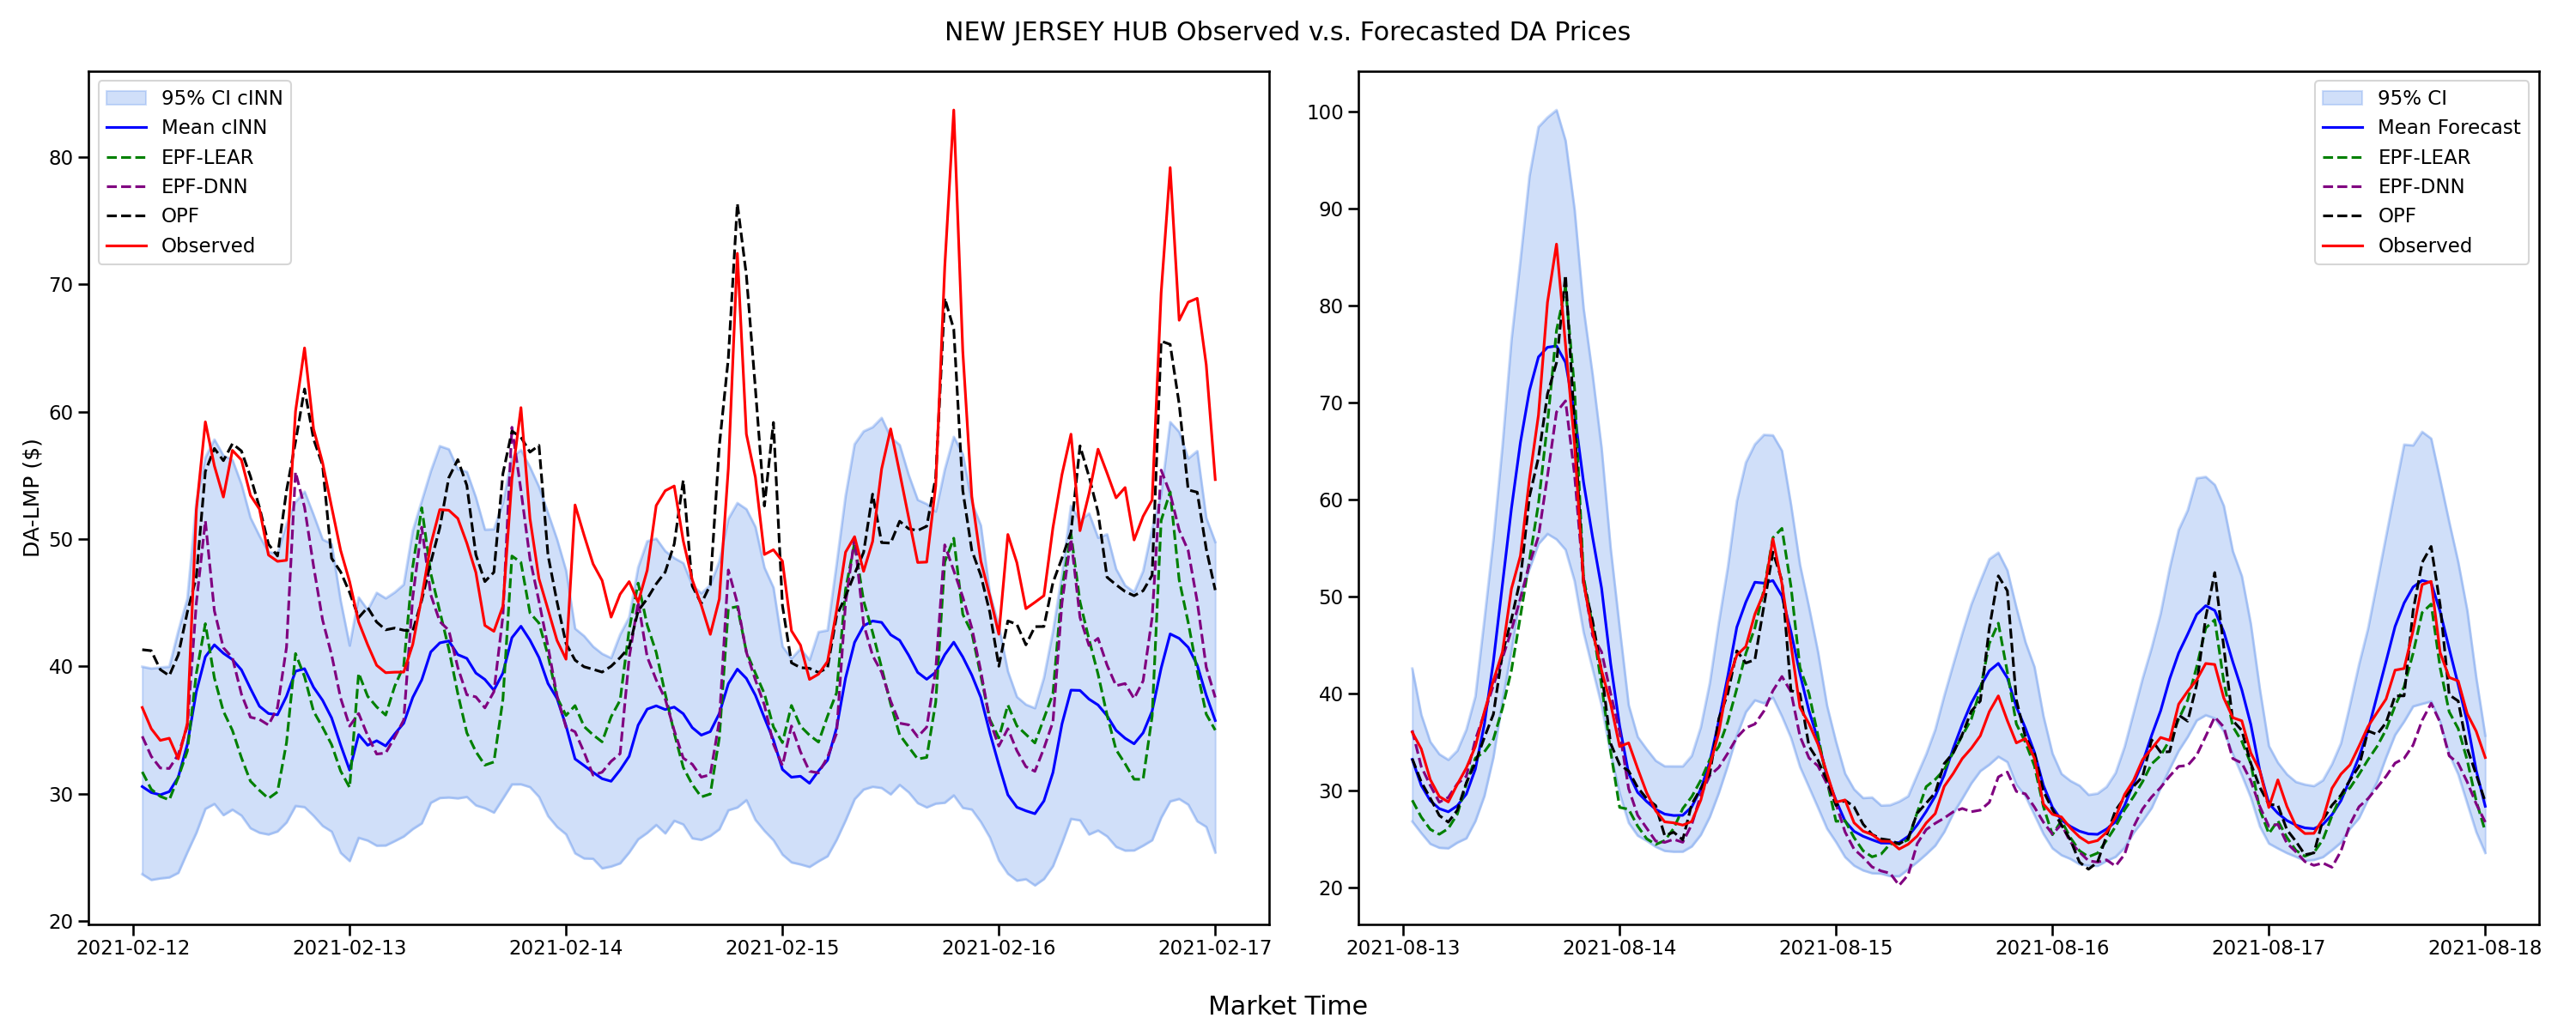
\includegraphics[width=150mm]{figs/nj_hub_ts}
%        }
    \end{center}
    \label{fig:forecast_timeseries}
\end{figure}

\begin{figure}[htbp]
    \caption[Comparison of forecasts at select market-hours]{
        Forecasts for our proposed probabilistic forecasting methodology and EPF-LEAR, EPF-DNN, and OPF baselines
        against the true DA prices are shown at the NEW JERSEY HUB price node over four hours in a single market day.
    }
    \begin{center}
        \setlength{\fboxsep}{0pt}%
        \setlength{\fboxrule}{1pt}%
%        \fbox{
        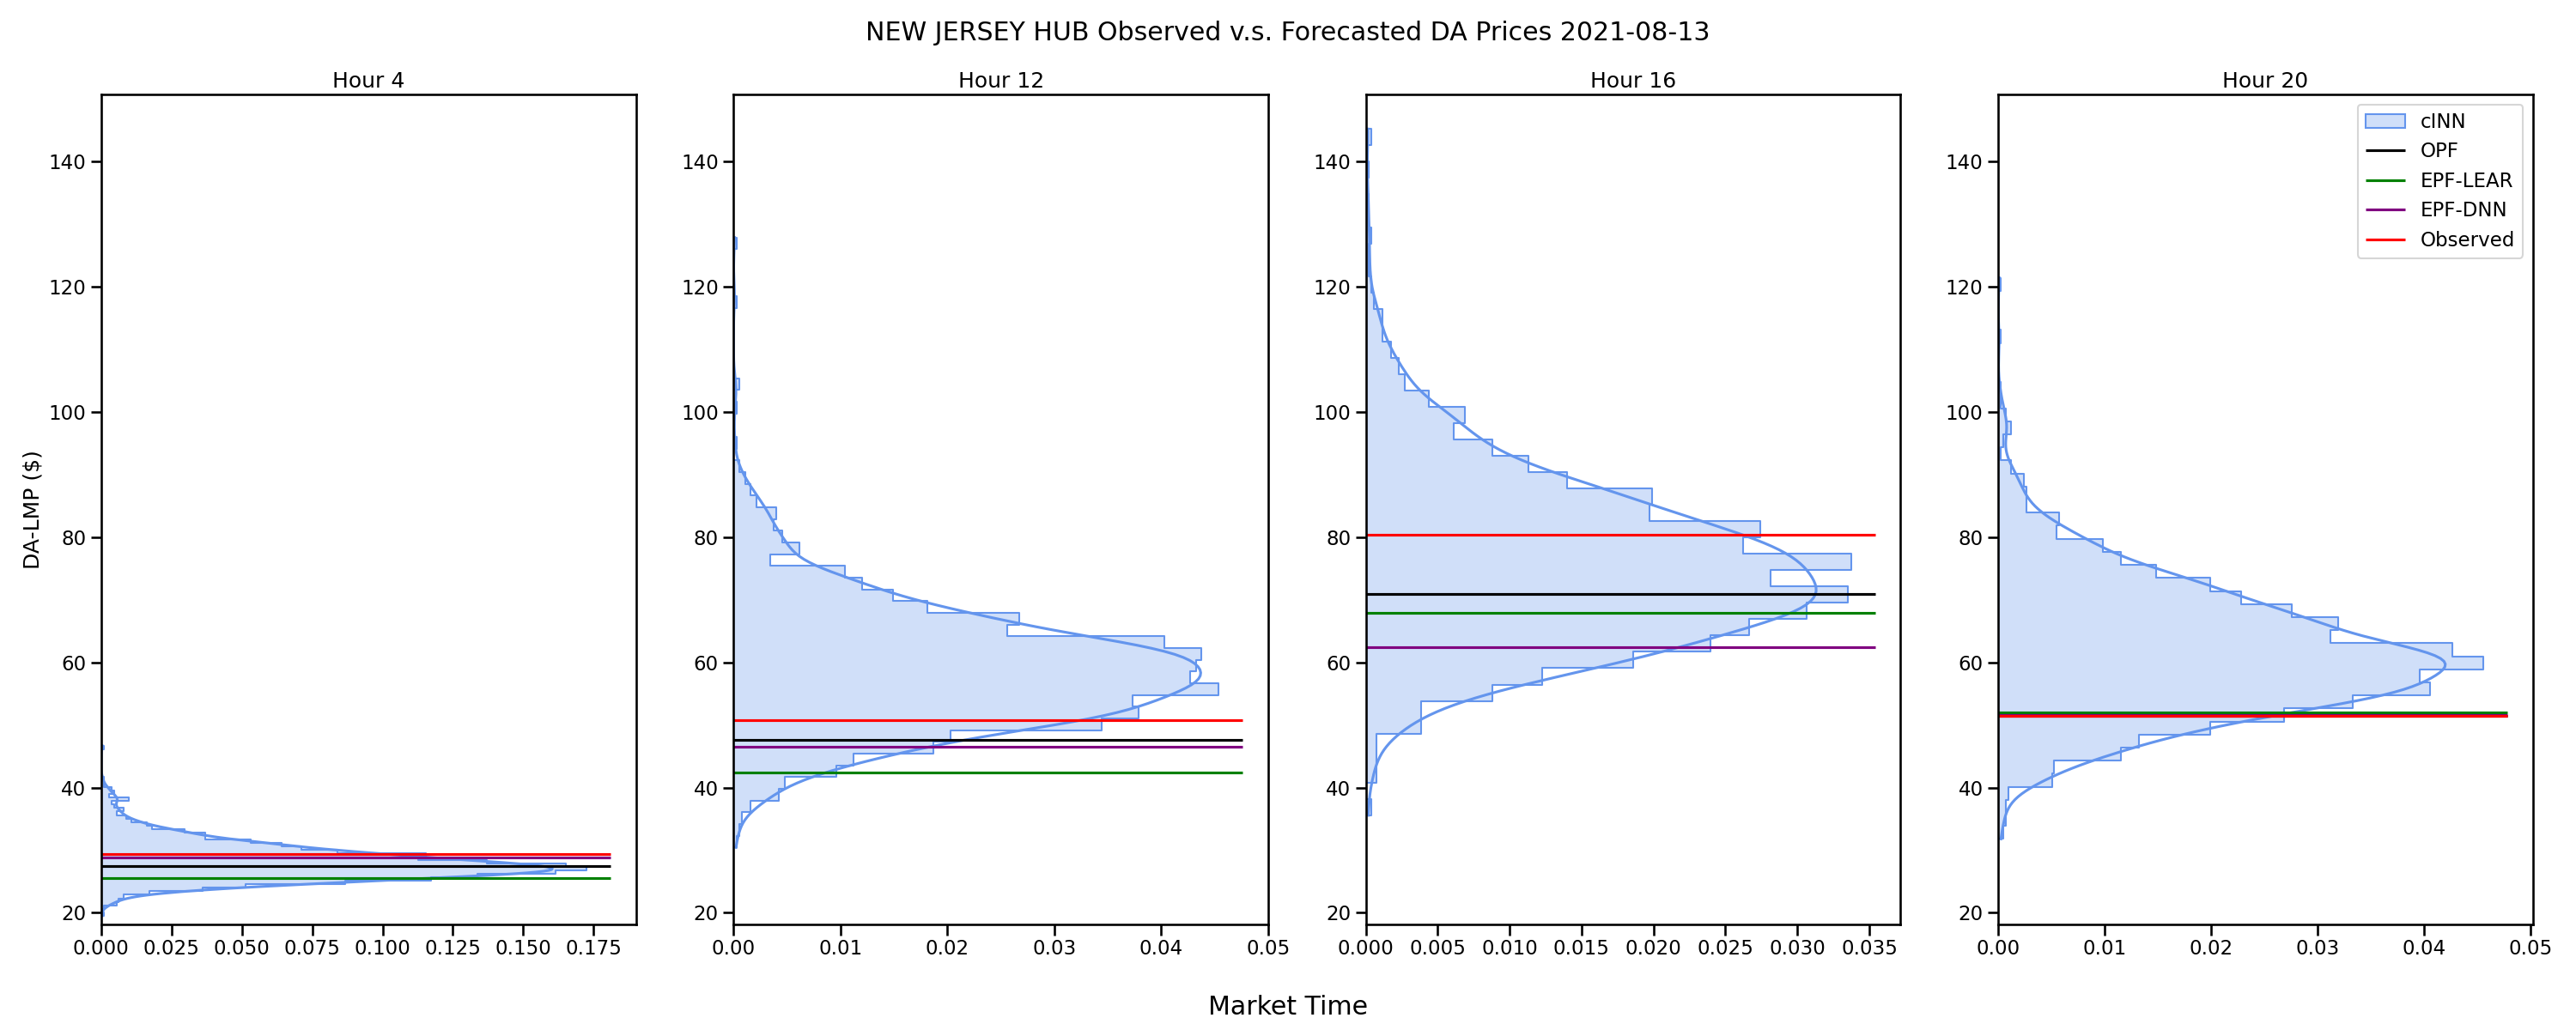
\includegraphics[width=150mm]{figs/nj_hub_densities}
%        }
    \end{center}
    \label{fig:univar_dens}
\end{figure}
